\section{Base decomposition: why the fit fails}
\label{app:decomp}

Sweeping $K \in \{2,4,8,16,32,64\}$ fits $T(K) = \kfitBase + \kfitSlope
\cdot K$ with $R^2 = \kfitRsq$. Latency saturates above $K{=}16$, so the
intercept is not interpretable as a floor. Two measurement-based bounds
constrain the split instead: from $T(2) = 202$\,ms the floor is at most
$53\%$ of the base; from the canvas step denoising is at least $32\%$.
Linear interpolation narrows this to prefill $\approx 38\%$, denoising
$\approx 62\%$. Figure~\ref{fig:ksweep} shows the saturation that
makes the intercept uninterpretable.

\begin{figure}[!htbp]
\centering
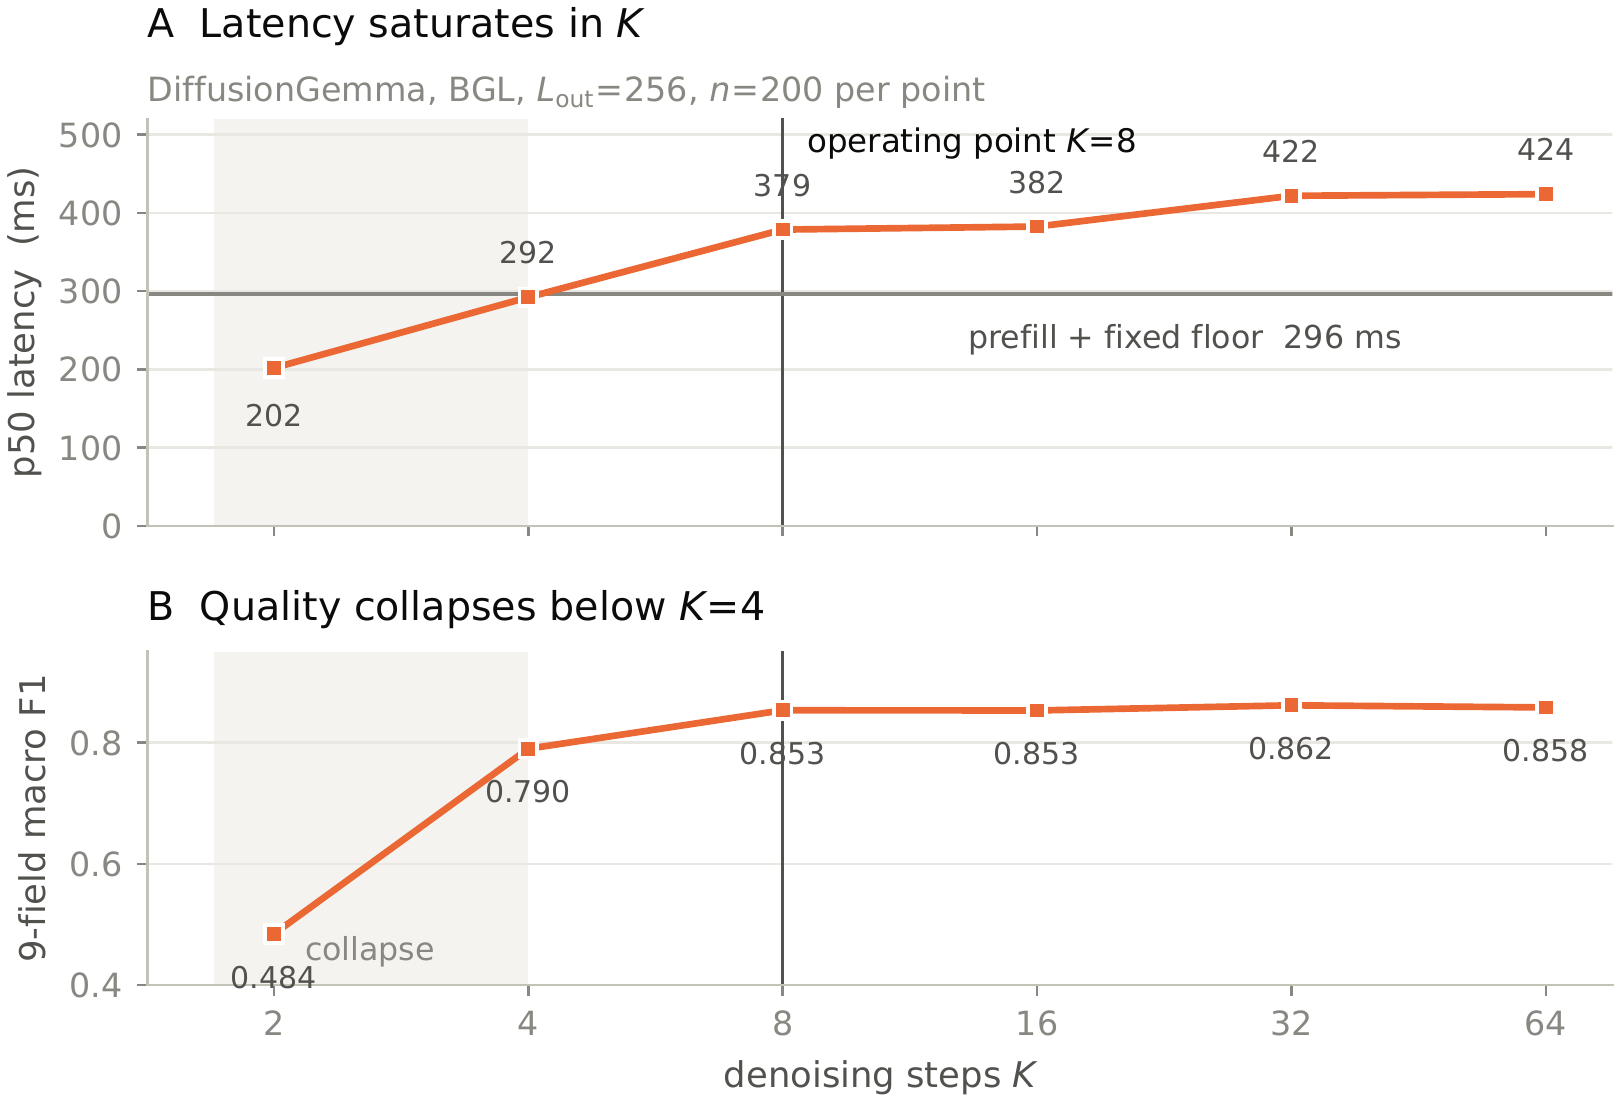
\includegraphics[width=0.85\linewidth]{figures/fig4_ksweep_hires.png}
\caption{Denoising-step sweep at $L_{\mathrm{out}}{=}\canvasLength$
(BGL, $n{=}200$). Latency saturates above $K{=}16$; quality is flat
above $K{=}8$.}
\label{fig:ksweep}
\end{figure}
